\chapter{Testování}
\label{sec:te}

\section{Automatizované testy}

K~aplikaci jsem vytvořil sadu automatizovaných testů, které ověřují funkčnost jednotlivých komponent. Konkrétně jde o~testy pro \textit{model} aplikace (zde je testována především třída \texttt{Garage}), webové rozhraní a API systému. Tyto testy byly implementovány pomocí frameworku pytest \cite{pytest}.

Části aplikace, u~kterých je automatizované testování problematikcé, jako například funkce využívající APScheduler (viz sekce \ref{sec:im_scheduler}) nebo zasílání e-mailů, jsem otestoval ručně.

\subsection{Testovací konfigurace}

Před spuštěním automatizovaných testů je nutné upravit konfiguraci aplikace. Především je třeba určit umístění testovací databáze a souboru s~uživatelským nastavením. Tyto soubory jsou v~průběhu testů upravovány a po dokončení smazány.

Také je nutné vypnout ochranu proti CSRF v~celé aplikaci, což výrazně zjednodušší testování formulářů aplikace. Jelikož požadavky s~metodou \texttt{post} vytvořené v~testech nepocházejí z~webových stránek aplikace, nemohou dodat CSRF \textit{token}, který je součástí formuláře. 

Sdílení \textit{tokenu} mezi aplikací a testy by sice bylo možné implementovat, bylo by však zbytečně komplikované. Za vhodnější postup považuji vypnutí CSRF ocharny pro většinu testů a funkčnost ochrany otestovat v~samostatném testu (viz sekci \ref{sec:te_csrf}).

Změna konfigurace aplikace je provadena nastavením proměnné prostředí \texttt{GARAGE\_SYSTEM\_CONFIG} na soubor s~testovací konfigurací (blíže viz sekci \ref{sec:im_config}).

\subsection{Testování \textit{modelu}}
\label{sec:te_model}

Testování \textit{modelu} aplikace spočívá především v~testování metod třídy \texttt{Garage}. Třída \texttt{Event} slouží pouze k~uchování dat o~události a neimplementuje žádné metody, které by bylo možné testovat.

Testovány jsou následující scénáře:

\begin{itemize}
    \item Přidání garáže.
    \item Smazání garáže.
    \item Kontrola zmeškaných hlášení.
    \item Zaslání kontrolího hlášení.
    \item Změna stavu po zaslání události.
    \item Zneplatnění API klíče.
\end{itemize}

Zde stojí za zmínku test kontroly zmeškaných hlášení. V~něm je garáži zasláno kontrolní hlášení, čímž je určen čas dalšího očekávaného hlášení. Po překročení tohoto času je potřeba otestovat, zda byl stav garáže změnen na \uv{Nehlásí se}.

Jelikož je minimální perioda hlášení 1 minuta, prosté čekání (například pomocí funkce \texttt{sleep()}) by proces testování neúnosně zpomalilo (pro srovnání spuštění všech testů aplikace na běžném počítači zabere asi 4 sekundy). Vhodnější je tedy časový posun nasimulovat.

K~tomu je použita knihovnu FreezeGun \cite{freezegun}. Tato knihovna umožňuje explicitně nastavit datum a čas, které vrátí funkce \texttt{now()}, používaná v~implementaci třídy \texttt{Garage}. Použití knihovny při testování kontroly promeškaných hlášení je demonstrováno v~ukázce \ref{lst:freezegun}.

\begin{listing}[htbp]
\caption{\label{lst:freezegun} Test kontroly promeškaných hlášení. Pomocí knihovny FreezeGun je čas nastaven na půlnoc 1. 1. 2011. Poté je čas posunut o~dvě hodiny a otestována změna stavu garáže}
\begin{minted}[bgcolor=codebg]{python}
from freezegun import freeze_time

# všechna volání datetime.datetime.now()
# pocházející z~této funkce vrátí
# hodnotu 2011-01-01 00:00:00
@freeze_time("2011-01-01 00:00:00")
def test_check_report(garage):
    new_garage = garage.add_garage()
    new_garage.period = 60 # explicitní nastavení periody
    new_garage.add_report_event()
    new_garage.check_report()

    assert new_garage.state == garage.STATE_OK

    # nastavení návratové hodnoty funkce now()
    # v~rámci bloku with
    with freeze_time("2011-01-01 02:00:00"):
        new_garage.check_report()
        assert new_garage.state == garage.STATE_NOT_RESPONDING
\end{minted}
\end{listing}

\subsection{Testování API}

Testy API nadřazeného systému ověřují funkčnost následujících operací:

\begin{itemize}
    \item Vytvoření garáže při vypnutném reg. módu.
    \item Zaslání události.
    \item Zaslání události s~neplatným API klíčem.
\end{itemize}

U~každého testu je zkontrolováno, zda byla odeslána správná odpověď na příslušný požadavek -- návratový kód (například \textit{404 -- Forbidden}) a zaslaná data. Je tedy testována pouze reakce API \textit{controlleru}, vliv operací na databázi nadřazeného systému je pokryt v~testu \textit{modelu} (viz sekci \ref{sec:te_model}).

\subsection{Testování webového rozhraní}

V~těchto testech je zkoumán \textit{controller} webového rozhraní a zobrazované HTML stránky. Testovány jsou tyto scénáře:

\begin{itemize}
    \item Zobrazení hlavní stránky.
    \item Zobrazení stránky garáže.
    \item Zobrazení událostí.
    \item Zobrazení chybové stránky při zadání neexistující garáže.
    \item Úprava dat garáže (označení a poznámka).
\end{itemize}

V~každém testu je testováno, zda aplikace v~reakci na požadavek vygeneruje odpovídající webovou stránku a vrátí odpovídající návratový kód.

Zobrazení testovaných stránek vyžaduje přihlášení do webového rozhraní nadřazeného systému. To by vyžadovalo zaslání přihlašovacího požadavku se správným heslem před spuštěním testů.

Další možnost je nastavit přihlášení explicitně, modifikací testovací HTTP relace. Díky tomu není nutné spoléhat na funkcionalitu přihlašování, která je testována samostatně.

Framework Flask umožňuje k~aplikaci vygenerovat testovacího klienta, jehož relaci je možné libovolně modifikovat \cite{flask_testing}. Díky tomu lze nastavit proměnnou \texttt{logged\_in}, která je používána ke kontrole přihlášení (viz sekci \ref{sec:im_auth}). Nastavení této proměnné je provedeno následujícím způsobem:

\begin{listing}[htbp]
\caption{\label{lst:logged_in} Explicitní nastavení proměnné \texttt{logged\_in} na požadovanou hodnotu. Pomocí takto modifikovaného testovacího klienta lze zasílat požadavky, na které bude aplikace reagovat jako při přihlášení}
\begin{minted}[bgcolor=codebg]{python}
# app_client je testovací klient Flask aplikace
# získaný pomocí metody test_client()
def set_logged_in(app_client, value):
    with app_client as c:
        with c.session_transaction() as s:
            s['logged_in'] = value
\end{minted}
\end{listing}

\subsection{Testování autentizace uživatele}

Toto testování ověřuje jednak funkci \textit{controlleru} provádějícího autentizaci, jednak přístup k~souboru s~uloženým otiskem hesla. Jsou zde testovány tyto scénáře:

\begin{itemize}
    \item Zobrazení přihlašovací stránky.
    \item Kontrola přihlášení při přístupu k~dalším částem systému (viz sekci \ref{sec:im_auth}).
    \item Přihlášení pomocí implicitního hesla.
    \item Odhlášení.
    \item Změna hesla.
\end{itemize}

Opět jsou kontrolovány návratové kódy odpovědí. Také je testováno, zda byla provedena příslušná přesměrování (například přesměrování na přihlašovací stránku při pokusu o~přístup k~částem rozhraní bez přihlášení) a zobrazení chybových hlášek (například při zadání neplatného hesla).

\subsection{Testování ochrany proti CSRF}
\label{sec:te_csrf}

Jelikož byla u~předchozích testů vypnuta ochrana proti CSRF, je vhodné provést ještě jednoduchý test, který ověří její fungování. Zde stačí zaslat testovanému formuláři data pomocí metody \texttt{post} bez platného CSRF \textit{tokenu}.

Výchozí chování CSRF ochrany ve frameworku Flask je v~případě chybějícího nebo neplatného \textit{tokenu} zaslat návratový kód \textit{400 -- Bad request} \cite{flask_wtf}. V~těle odpovědi je pak informace o~problému s~\textit{tokenem}. Stačí tedy otestovat návratový kód a obsah odpovědi (viz ukázka \ref{lst:csrf_test}).

\begin{listing}[htbp]
\caption{\label{lst:csrf_test} Test ochrany proti CSRF}
\begin{minted}[bgcolor=codebg]{python}
def test_csrf():
    ...
    # vypnutí ochrany proti CSRF
    app.config['WTF_CSRF_ENABLED'] = True
    app.config['WTF_CSRF_CHECK_DEFAULT'] = True

    # zaslání požadavku na přihlášení bez platného tokenu
    response = app.test_client().post('/login', data={
        # na zaslaném hesle nezáleží
        # žádost bude odmítnuta na základě neplatného tokenu
        'password' : 'test password',
        'csrf_token' : 'some fake token'
        })

    assert response.status == '400 BAD REQUEST'
    # odpověď by měla zmiňovat CSRF
    assert 'CSRF' in response.data.decode('utf-8')
\end{minted}
\end{listing}


\section{Testovací nasazení aplikace}

V~rámci testování jsem se rozhodl nasadit aplikaci nadřazeného systému na virtuálním serveru, způsobem popsaným v~sekci \ref{sec:an_cloud}. Tím je jednak otestován průběh nasazování aplikace, jednak je běžící aplikaci možné použít pro demonstrační účely. Aplikace je momentálně\footnote{Aplikace byla spuštěna 30. 3. 2018. Jelikož je registrace domény platná do 30. 6. 2018, bude její provoz po tomto datu ukončen.} přístupná na doméně \url{https://demo-garaze.tk}.

Jelikož je aplikace dostupná z~internetu, není vhodné použít k~provozu HTTPS \textit{self-signed} certifikát. Místo toho je k~doméně registrován platný certifikát autority Let's Encrypt.

Aplikace k~provozu využívá server Apache. Při konfiguraci HTTPS na tomto serveru jsem vycházel z~článku \textit{Strong SSL Security on Apache2} \cite{apache_ssl}. Správnost konfigurace a platnost certifikátu byla ověřena pomocí testu poskytovaného společností Qualys. Výsledné hodnocení je možné vidět na obrázku \ref{fig:ssl_test}.

\begin{figure}[h!]
    \centering
    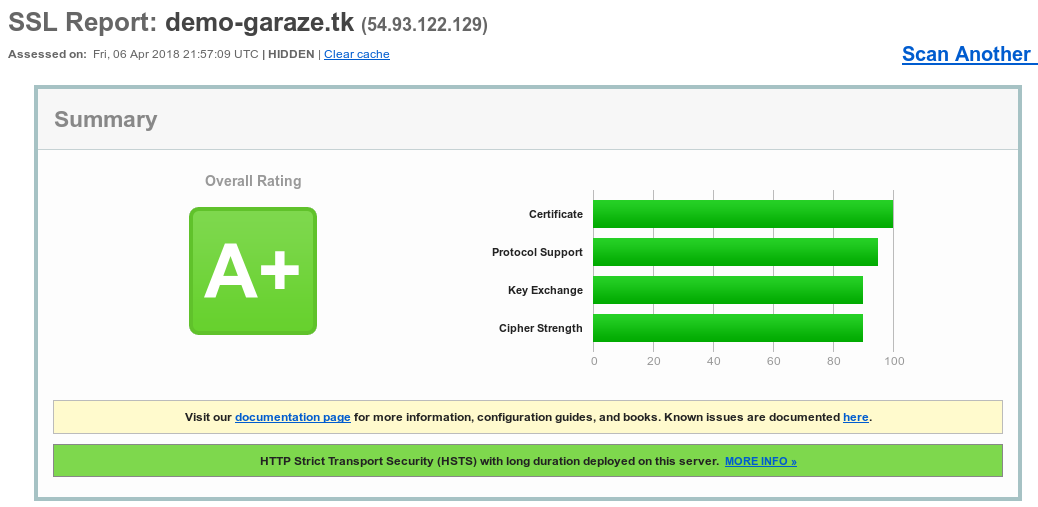
\includegraphics[width=\textwidth]{images/ssl_test.png}
    \caption[Výsledky testu HTTPS konfigurace]{Výsledky testu HTTPS konfigurace poskytnutného společnstí Qualys.}
    \label{fig:ssl_test}
\end{figure}

% napsat ze sme pri nasazovani prisli na novy chyby, ktery nebyly na lokale videt -- to s tim vodhlasovanim a secret_key, a to ze apache zahazuje ty headery s nepovolenejma znakama
Nasazení aplikace v reálném prostředí odhalilo několik chyb, které nebyly při lokálním testování patrné. V první řadě se ukázalo, ze server Apache od verze 2.4 ignoruje v příchozím požadavku hlavičky, které obsahují podtřžítka (\texttt{\_}) \cite{apache_headers_update}.

% v tyhle kapitole taky poresit to ze se jako bottleneck ty komunikace zda bejt ten https handshake a ze by se to asi dalo vyresti pouzitim sessions na strane klienta http://docs.python-requests.org/en/latest/user/advanced/#session-objects -- tohle spis v ty sekci co bude testovat vykon rpi